\documentclass[12pt]{article}
\usepackage[utf8]{inputenc}
\usepackage[sfdefault]{carlito}
\renewcommand{\baselinestretch}{1.5}

\usepackage{float}
\usepackage[a4paper,hmargin=1.5cm,vmargin=2cm]{geometry}
\usepackage{graphicx}
\usepackage{amsfonts}
\usepackage{textcomp}
\usepackage{hyperref}
\usepackage{listings}
\usepackage{array}
\usepackage{tabularx}
\usepackage{mathtools}
\usepackage{longtable}
\usepackage{enumitem}
\usepackage{caption}

% parsep is interlinia
\setitemize{noitemsep,topsep=5pt,parsep=0pt,partopsep=0pt}
\setenumerate{noitemsep,topsep=5pt,parsep=0pt,partopsep=0pt}

\usepackage[backend=bibtex,sorting=ydnt]{biblatex}
\bibliography{thesis-tex/bibliography.bib}


\usepackage{wrapfig}
\graphicspath{{figures/}}

\usepackage{chngcntr}
\def\mych{\counterwithin{figure}{chapter}\chapter}
\def\mysec{\counterwithin{figure}{section}\section}
\def\mysubsec{\counterwithin{figure}{subsection}\subsection}
\def\mysubsubsec{\counterwithin{figure}{subsubsection}\subsubsection}

\title{
{\small Ewa Czechowska } \\
\bf\textit{ Master’s Thesis - TODO replace me } \\
\vspace{4cm}}
\date{\today}


\begin{document}

\maketitle
~\vspace{8cm}
\newpage

\tableofcontents
\newpage

% 1
\section{Introduction}

% this should take 2 or 3 pages;
% the subsections are not mandatory

\subsection{Topic and problem description}

Microservices, Continuous Integration and Delivery, Docker, DevOps, Infrastructure as Code - these are the current trends and buzzwords in the technological world of 2020. A popular tool which can \textbf{facilitate the deployment and maintenance of microservices is Kubernetes}. Kubernetes is a platform for running containerized applications, for example: microservices. The first part of the problem, which this thesis is trying to solve is: \textbf{how to deploy Kubernetes itself}. The second part is: how to ensure that the deployment fulfills the needs of a production environment.

Any application may comprise several components, for example: a backend server, a frontend server, database. It is common knowledge, that deploying an application to a production environment, should obey a set of guidelines. It should be easy to view all the log messages generated by each of the components of the application, the application should be reachable for its end users and also, it would be nice if in a case of any component failure - that component should be available despite the failure. \textbf{Kubernetes facilitates satisfying such requirements. But, the aim of this thesis is to ensure such requirements for Kubernetes itself}. A set of requirements will be selected. Then, several ideas will be provided on how to meet each of the chosen requirements.

\textbf{There are plenty methods of Kubernetes cluster deployment. Many will be described}. The methods differ in relation to: how much customization they offer, which clouds they support, how much they cost. Some of the methods has existed since the Kubernetes was created, the other ones, like AWS EKS, has been invented later. The latter methods are harder to find in books tackling the Kubernetes deployment task, but there are other sources which explain how to use them (mostly: official documentation of the methods and blog posts).

There exist sources which compare several methods of Kubernetes cluster deployment. But, they are either non-formal sources (e.g. blog posts or Internet tutorials) or they do not compare the two methods selected in this thesis or they do not consider the production environment. Therefore, \textbf{this thesis has the opportunity to offer some novelty}.

\subsection{Aim and scope of this study}


Nowadays, the world is full of choices. The technology is exuberant. However, time, as our resource, is limited. Thus, it is often advisable to use an already existing solution instead of inventing our own. It is even better if there are many such solutions. The presented Master's thesis aims \textbf{to compare two methods of deploying a Kubernetes cluster}. Both of the methods concern AWS cloud. AWS cloud was chosen mainly because of its wide popularity and the range of provided services. Besides the two chosen methods of deployment, there are many more, including the DIY method and deploying on-premises.

This thesis attempts \textbf{to stipulate the requirements of a production environment}. Then, the requirements are used as comparison criteria to help assess the two methods of deployment. It is expected that one method could be easier to use than the other but also a method could be insufficient to satisfy all the production environment requirements. Furthermore, other criteria will be used, such as: cost of both methods and amount of problems encountered.

It is intended, that this work should \textbf{focus on the practical aspect of a Kubernetes cluster deployment}. The limitations and known issues of both methods are going to be described. Therefore, the thesis might be helpful to the engineers or consultants who are responsible for Kubernetes cluster deployment.

There are already some literature sources that compare chosen methods of Kubernetes cluster deployment. However, they are not constructed in a scientific, formal form (they are either blog posts or tutorials available in the Internet) or they do not consider a production environment.

\subsection{Structure of this thesis}

The presented thesis is divided into seven chapters.

The first chapter is \textbf{an introduction}. It describes briefly the topic and the problem. Then, it includes aim and scope of this study. And then, the structure of this study is presented.

The second chapter focuses on \textbf{basic information concerning: microservices, DevOps, Docker and Kubernetes}. Furthermore, AWS cloud is described there. The chapter ends with stipulating the requirements of a production deployment.

In the next, third, chapter \textbf{the most popular methods of Kubernetes cluster deployment are described}. The two methods that will be compared in the later part are also included.

The fourth chapter is a practical one. It provides \textbf{planning and designing of the production deployment} which will be conducted later in the thesis. Some important decisions are taken here, for example: which Kubernetes version to use or which tools to use.

Then, the fifth chapter \textbf{refers to code} and it is the core part of this Master's thesis. It provides \textbf{the steps that were used to deploy Kubernetes clusters on AWS, using two methods}:
\begin{enumerate}
\item deployment on AWS EKS service,
\item deployment with Kops on AWS EC2 instances.
\end{enumerate}
Anyone following these steps should be capable to recreate the same Kubernetes clusters as described here and thus, it should be possible to draw the same conclusions as the author of this thesis did. Furthermore, all the encountered problems and suggested solutions are provided.

The sixth chapter \textbf{presents the comparison} of the two deployment methods using chosen comparison criteria. Each subsection of this chapter deals with a single comparison criterion.

Finally, the last, seventh, chapter offers \textbf{the summary}, briefly describes the lessons learned and also provides some ideas for future work.

\newpage

% 2
\mysec{From microservices to automated orchestration}
\textit{This chapter serves as an introduction to microservices, DevOps, Docker, Kubernetes and AWS. It is a theoretical chapter. It ends with stipulating the requirements of a production deployment.}

\subsection{Microservices, DevOps, Continuous Delivery and Infrastructure as Code}
\textit{This subchapter attempts to briefly explain a set of terms which will be used throughout this Master's thesis.}


\subsubsection{Microservices}
Microservices may be defined as a \textbf{cloud-native architecture} which aim is to provide software systems as a package of small services. Each of these small services should be \textbf{independently deployable} and also each of them could utilize a different technological stack and platform. The services run in separate processes and communicate with each other through mechanisms like: RESTful APIs \cite{article-micro-devops} because they utilize the language-agnostic protocol: HTTP \cite{book-pr-devops}.

Another definition of microservices is: "a microservice is simply \textbf{a self-contained service that does one thing}. If you put enough microservices together, you get an application" \cite{book-cndwk}.

Microservices are often presented as an alternative to and compared to \textbf{monoliths}. For instance, the author of "Practical DevOps" \cite{book-pr-devops} explains that, in comparison to monoliths, microservices have more integration points and suffer from a
higher possibility of failure. Furthermore, in \cite{book-cndwk} it is written that:
\begin{itemize}
\item monoliths are hard to scale, both in terms of code and also in terms of teams of people,
\item monoliths are easier to understand, because the code can be found in one place.
\end{itemize}

The schema presented in figure ~\ref{fig:microservices-vs-mono} should help to illustrate the difference between two software architecture styles.
\begin{figure}[H]
    \centering
    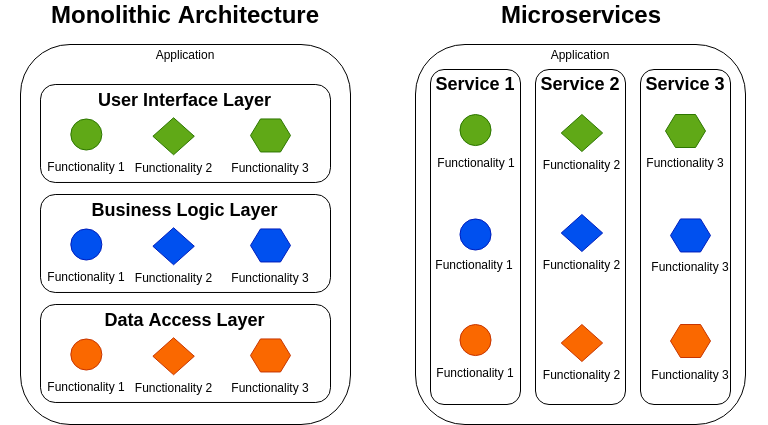
\includegraphics[width=10cm]{figures/microservices-vs-mono.png}
    \captionsetup{justification=centering,margin=2cm}
    \caption{The difference between two software architecture styles: monolith and microservices \cite{online-trans-mono-micro}}
    \label{fig:microservices-vs-mono}
\end{figure}

Microservices are not a panacea \cite{book-cndwk} and not a silver bullet \cite{article-micro-devops}, but in order to design a great software system, one should be acquainted with many solutions.

\subsubsection{DevOps}
\textbf{DevOps} and microservices have been both increasingly drawing attention since 2014, according to Google Trends. DevOps can be applied to both: monoliths and microservices, but using it for microservices promotes the importance of small teams. DevOps may be explained as a set of practices which aims \textbf{to decrease the time from the point of introducing a change to a point when the change is transferred to the production environment}. DevOps also focuses on maintaining the software quality in terms of both: code and the delivery process \cite{article-micro-devops}.

Moreover, DevOps can be defined as: "a movement to reduce barriers and friction between organizational silos - development, operations, and other stakeholders involved in planning, building, and running software". The definition continues, that even though the most visible aspect of DevOps may be technology, it is \textbf{culture, people and processes which have the most impact on flow and effectiveness} \cite{book-iac}. DevOps, as a movement, has its roots in the \textbf{Agile Manifesto}. It can be said, that DevOps obeys the first rule of the mentioned Agile Manifesto: "Individuals and interactions over processes and tools" \cite{book-pr-devops}.

In "Practical DevOps" \cite{book-pr-devops}, it is explained that DevOps spans several disciplines. Both: technical and soft skills are required to incorporate the DevOps movement. The word: \textbf{"DevOps" comes from combining: "development" and "operation"}. This already may indicate, that DevOps is a practice where collaboration between many teams matters and is encouraged.

\subsubsection{Continuous Integration and Continuous Delivery}
There are many DevOps practices: forming small teams, but also \textbf{automation and Continuous Integration (CI) and Continuous Delivery (CD)} \cite{article-micro-devops, book-pr-devops}. The first time that CI was written about was by Kent Beck in the book: "Extreme Programming Explained". CI was introduced to the world as Extreme Programming practice. The idea behind it was \textbf{to continuously --- meaning very often --- verify a source code}. CI represents a paradigm shift, because without CI, a software may be deemed broken unless somebody proves otherwise. With CI, a software is proven to work with every change added to source code \cite{book-cicd}.

There are many advantages of using CI \cite{book-cicd}:
\begin{itemize}
\item CI helps to identify the change in a source code that resulted in failing tests,
\item bugs may be caught earlier in the delivery process which is cheaper and faster when compared to fixing them in already deployed production environment,
\item delivery process is automated, thus human error is limited,
\item delivery process is automated, thus it is repeatable and easily reproducible,
\item delivery process is clearly stipulated in code,
\item CI helps different team members to communicate \cite{bachelor-ha}.
\end{itemize}

In order to incorporate the practice of Continuous Integration, a \textbf{Continuous Integration server} is needed. Examples of such a server are: Jenkins \cite{online-jenkins}, GoCD \cite{online-gocd}. The second ingredient needed is \textbf{a CI pipeline}. A CI pipeline consists of several stages which provide steps, to be performed, in order to release the software. There may be a lot more stages, for instance: the test stage can be split into many stages, each running different kind of tests (integration, functional, non-functional, acceptance, etc.) \cite{bachelor-ha, book-cicd}. The pipeline starts with a user uploading their code onto a version control system. A CI server should pick up a change and initiate the pipeline run \cite{book-pr-devops}. An example pipeline is illustrated in figure ~\ref{fig:pipeline}.

\begin{figure}[H]
    \centering
    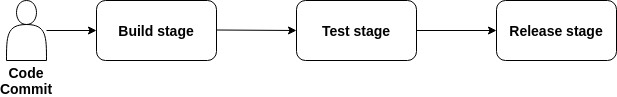
\includegraphics[width=14cm]{figures/pipeline.png}
    \captionsetup{justification=centering,margin=2cm}
    \caption{A simple example CI pipeline, consisting of a few stages, starting with a developer uploading a change of code}
    \label{fig:pipeline}
\end{figure}

Each stage of a pipeline may be either passed or failed. The failed stage indicates that some particular code change cannot satisfy the requirements of that particular stage. The stages are run in a specific order. In figure ~\ref{fig:pipeline}, the order is demonstrated with arrows. The first stage is build, then test, then release. Should the build stage fail, then neither the test nor the release stage will be run.

There exists an extension of continuous integration and it is called: \textbf{Continuous delivery (CD)}. CD verifies that a piece of software is always in a deployable state. CD is thus even more attractive than CI, because it offers even more automation \cite{online-do-cicd}.

\subsubsection{Infrastructure as Code}
Together with automation and DevOps there comes the term: \textbf{Infrastructure as Code (IaC)}. IaC may be understood as an approach to automate the infrastructure based on practices from software development. Consistent and repeatable routines are encouraged for infrastructure provisioning and configuration. There are three core practices required to implement IaC: \textbf{define everything as code} (e.g. the configuration can be saved as YAML files), \textbf{continuously validate the code} and, \textbf{build a system from small, loosely-coupled pieces} \cite{book-iac}.

Back in time, developers dealt with software, while operations teams worked on hardware and the operating systems. Now, the hardware is in the cloud and thus, it can be handled in the same way as software. \textbf{The DevOps movement brings software development skills to operations}. It concerns both: tools and workflows \cite{book-cndwk}. The movement from deployment on-premises to the cloud also deserves a few words, but it will be handled in the subchapter: \ref{section-aws}.

\subsection{AWS - The Amazon Cloud} \label{section-aws}
\textit{This subchapter offers an introduction to cloud computing and AWS cloud and also the explanation why this particular cloud was chosen.}
\\

There are three revolutions going on \cite{book-cndwk}:
\begin{itemize}
\item the creation of the cloud,
\item the dawn of DevOps,
\item coming of containers.
\end{itemize}

These revolutions are interlinked and happen all at once. This subchapter focuses on the cloud revolution. The days of "bare-metal", before cloud, are referred to as \textbf{"Iron Age"} \cite{book-cndwk,book-iac}. The current times (after cloud was invented) are called \textbf{"Cloud Age"} and the cloud infrastructure - \textbf{Infrastructure as a Service (IaaS)}. IaaS allows to outsource not only the hardware but also the software. The outsourced software involves: operating systems, networking scripts, monitoring logic etc. \textbf{Managed services} can take care of many non-functional requirements. There is no more grand upfront investment. Having a large-scale system to build may have cost a fortune in the past. Back then, the computing power was a capital expense and now --- it is an operational one. Now, there is no fixed cost and the expense depends most often on cloud resources utilization \cite{book-cndwk, article-aws-architecting}.

\textbf{Cloud computing} may be defined as a model that provides end users with access from any device, as long as the device has an Internet access, to a shared set of cloud resources. The cloud resources involve various servers and services. Taking a step away, there may be differentiated four \textbf{deployment models}: private cloud, community cloud, public cloud, hybrid cloud. Private cloud means that the software is deployed on-premises, locally. Apart from that, there are also \textbf{service models}, which the most popular are \cite{article-poni-cloud}:
\begin{itemize}
\item Infrastructure as a Service (IaaS),
\item Platform as a Service (Paas),
\item Software as a Service (Saas).
\end{itemize}

Public clouds like: Amazon AWS, Google Cloud Platform or Microsoft Azure represent IaaS. In the Amazon whitepaper "Architecting for the Cloud" \cite{article-aws-architecting}, many \textbf{cloud computing benefits} are listed:
\begin{itemize}
\item near zero upfront infrastructure investment,
\item just-in-time infrastructure --- meaning that it is simple to scale the applications,
\item more efficient resource utilization --- resources can be reserved or required on demand (instantly),
\item usage-based costing --- users do not pay for allocated but unused infrastructure,
\item reduced time to market --- some jobs can be run parallely.
\end{itemize}

Furthermore, AWS offers \textbf{a highly reliable and scalable infrastructure} \cite{article-aws-architecting}, ensures \textbf{attractive SLAs} (e.g. AWS promises to keep a Monthly Uptime Percentage of at least 99.99\% for compute resources) \cite{online-aws-sla} and it is also \textbf{widely adopted and provides many various services} \cite{cncf-2019}. These are the reasons why AWS was chosen for this thesis. The charts in figures \ref{fig:cncf-aws-pop1} and \ref{fig:cncf-aws-pop2} present the popularity of AWS solutions.

\begin{figure}[H]
    \centering
    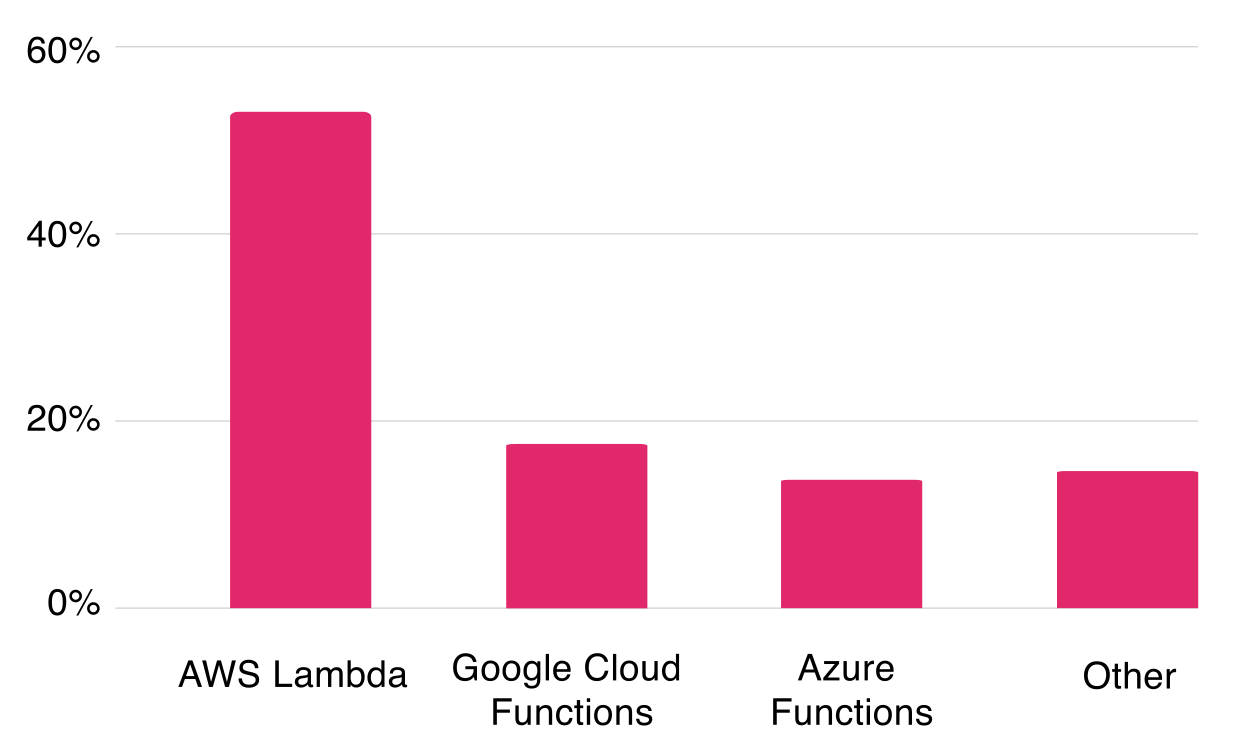
\includegraphics[width=8cm]{figures/cncf-aws-pop1.png}
    \captionsetup{justification=centering,margin=2cm}
    \caption{Hosted serverless platforms preferred by CNCF community during September and October 2019 \cite{cncf-2019}}
    \label{fig:cncf-aws-pop1}
\end{figure}
\begin{figure}[H]
    \centering
    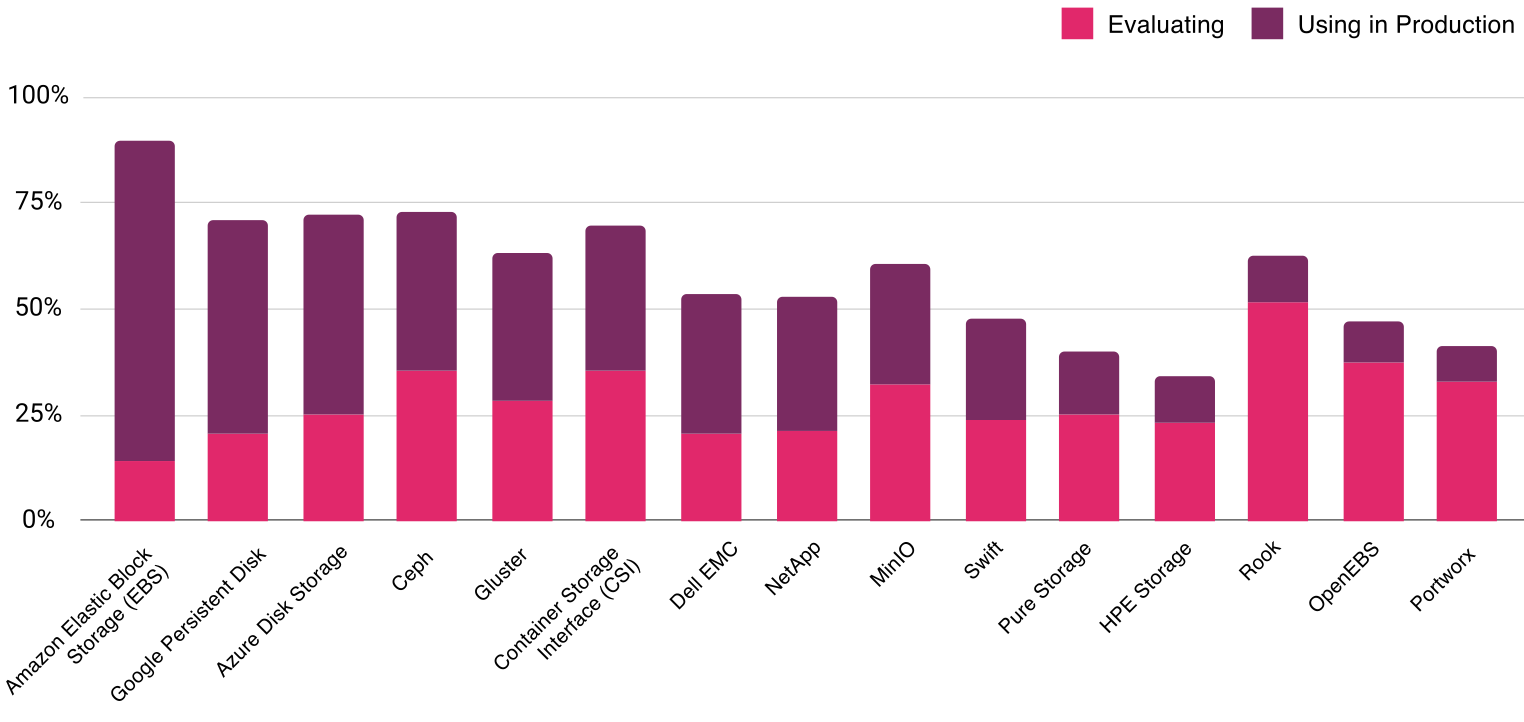
\includegraphics[width=13cm]{figures/cncf-aws-pop2.png}
    \captionsetup{justification=centering,margin=2cm}
    \caption{Cloud native storage preferred by CNCF community during September and October 2019 \cite{cncf-2019}}
    \label{fig:cncf-aws-pop2}
\end{figure}

\textbf{CNCF} is an abbreviation from \textit{Cloud Native Computing Foundation}. It is a non profit organization which fosters communities to support growth and health of cloud native open source software. CNCF adopts Cloud Native projects and catalogs them, depending on their maturity level. They also regularly conduct surveys concerning the Cloud Native and container-related technologies \cite{cncf-services}.



\subsection{Docker containers}
\textit{This subchapter provides an introduction to Docker containers and also compares them to Virtual Machines.}

In the old times, software was installed \textbf{on physical hardware directly}. Then, \textbf{virtualization and Virtual Machines (VMs)} were invented. The next great invention, after VMs, were \textbf{Docker containers}. In 2013 Docker was created as a standard way to manage containers\cite{book-devops-k8s}.

There are many advantages of using VMs and Docker containers in comparison to physical hardware. Docker containers and VMs:
\begin{itemize}
\item provide safer, isolated environment --- facilitate experiments,
\item are easier to automate, manage and replace,
\item provide reproducible environment,
\item limit "works on my machine" problem,
\item offer more security, e.g. an external user may have access only to a Docker container, not to a whole physical host,
\item have additional features, e.g. memory replication.
\end{itemize}

It is claimed, that containers may be replacing VMs. One reason for this might be that there is a significantly lower overhead in case of deploying containers compared to VMs \cite{article-modelling-performance-k8s}. Furthermore, in comparison to VMs, containers provide faster resource allocation. There are many implementation of containers, but among them, Docker is probably the most adopted \cite{article-state-machine}.

Docker uses some major Linux kernel features like: \textbf{namespaces and cgroups}. Namespaces control and limit the amount of resources a process can use, while cgroups manage the resources of a process group. They both help to provide isolation and resource limitation \cite{art-byza,book-devops-k8s}.

In order to be able to work with Docker containers, one has to know the \textbf{difference between a Docker container and a Docker image}. A Docker image is a read-only template. It has some software installed and configured. Each image has a name and a tag, which serves the same purpose as a software version. One image may be based on other image. There are many images available which are open-source and free, e.g. "debian:10.3" \cite{online-dh-debian}, "ubuntu:16.04" \cite{online-dh-ubuntu}. It is easy to build one’s own image, basing on the available images \cite{online-docker-doc}.

Below, there is an example of a source code which creates (builds) a Docker image. Just one file is enough for this task: \textbf{a Dockerfile} (listing \ref{lst:dockerfile}).

\begin{lstlisting}[basicstyle=\small,caption={A Dockerfile to build a Docker image with SSH server installed. Based on Docker official documentation \cite{online-docker-doc-bi}},captionpos=b,language=Bash,xleftmargin=0.3cm,label={lst:dockerfile}]
FROM ubuntu:16.04

RUN apt-get update && apt-get install -y openssh-server
RUN mkdir /var/run/sshd
RUN echo 'root:THEPASSWORDYOUCREATED' | chpasswd
RUN sed -i 's/PermitRootLogin prohibit-password/PermitRootLogin\
  yes/' /etc/ssh/sshd_config

# SSH login fix. Otherwise user is kicked off after login
RUN sed 's@session\s*required\s*pam_loginuid.so@session\
  optional pam_loginuid.so@g' -i /etc/pam.d/sshd

ENV NOTVISIBLE "in users profile"
RUN echo "export VISIBLE=now" >> /etc/profile

EXPOSE 22
CMD ["/usr/sbin/sshd", "-D"]
\end{lstlisting}

Docker containers are claimed to be \textbf{lightweight and portable}. Thus, containers are suitable for microservices. Since microservices are loosely-coupled, failure of one microservice should not affect other microservices of an application. This architectural style is characterized by fine granularity and therefore, it makes scaling more flexible and efficient \cite{article-k8s-as-avail}.

Docker containers are utilized by big companies like:  \textbf{Netflix or Twitter} \cite{article-nonf-twitter-netflix}. Docker is a technology described thoroughly in many literature sources and therefore there is no sense in repeating it. A curious reader is referred to read the official Docker documentation \cite{online-docker-doc}.

\subsection{Kubernetes as a Docker containers orchestration system}
\textit{This subchapter describes what Kubernetes is and what problems it solves. Furthermore, the chapter acknowledges Kubernetes popularity and briefly introduces chosen Kubernetes objects.}
~\\
~\\
The process of deploying multiple containers of one application can be optimized through automation. This kind of automation is referred to as \textbf{orchestration} \cite{art-byza}.

There was a need to automatically deploy and manage a large number of services at global scale on millions of servers. Thus, Google developed Borg. Borg is a private orchestration system. It is very powerful, but also very much coupled to Google’s own internal and proprietary technologies. Therefore, in 2014 Google launched a new project called: \textbf{Kubernetes}. The name comes from a Greek word which means "helmsman, pilot". Apart from Kubernetes, there are alternative solutions invented, other orchestrators, but Kubernetes \textbf{won the orchestration wars} \cite{book-cndwk,article-modelling-performance-k8s}.

"Kubernetes does the things that the very best system administrator would do: automation, failover, centralized logging, monitoring. It takes what we’ve learned in the DevOps community and makes it the default, out of the box." These are the words uttered by Kelsey Hightower --- a Google employee with legendary contributions to Kubernetes \cite{book-cndwk}.

Kubernetes was built \textbf{to make deployments easy, to reduce the time and effort} which needs to be poured into them. To achieve this goals, Kubernetes offers \textbf{a wide variety of features}\cite{k8s,book-cndwk,article-state-machine}:
\begin{itemize}
\item creating, destroying, replicating containers,
\item rolling updates of containers,
\item built-in health checks (liveness and readiness probes),
\item autoscaling,
\item redundancy and failover --- to make the applications deployed on top of Kubernetes more resilient and reliable,
\item being provider-agnostic --- Kubernetes can be deployed on-premises and in the cloud and in both cases it will provide the same set of features, thus, it may be said that Kubernetes unifies the underlying infrastructure,
\item utilizing provider-specific (sometimes referred to as: vendor-specific) features, e.g. AWS load balancer or Google Cloud load balancer,
\item self-healing,
\item service discovery,
\item load balancing,
\item storage orchestration.
\end{itemize}


Kubernetes is the first project of the CNCF \cite{article-state-machine}. Kubernetes is already \textbf{used by some well-known entities}, e.g. NASA \cite{nasa}, F-16 jets \cite{online-f16}, Zalando \cite{online-zalando}, ING \cite{online-ing}, booking.com \cite{online-bookingcom}. Apart from that, the \textbf{Kubernetes popularity is growing}, basing on the information from CNCF Survey 2019, which states that 78\% of respondents use Kubernetes in production and that this is a huge jump from 58\% using in the previous --- 2018 year \cite{cncf-2019}. Even the older CNCF Survey from year 2017 shows Kubernetes as number one cloud management platform --- it it presented in figure \ref{fig:cncf-con}.

The \textbf{basic working unit in Kubernetes is a pod}. A pod is an abstraction and it represents one application, a set of containers. Two things are crucial to know about pods \cite{article-modelling-performance-k8s}:
\begin{itemize}
\item all the containers defined in a pod will be deployed on one machine,
\item a pod has one IP address assigned and all the containers defined in this pod share the same IP address.
\end{itemize}

A pod is all that is needed to deploy a set of containers. Pod is a Kubernetes object and there are many more objects, for example: deployment, replica sets, service, ingress. The important thing to note is that these \textbf{objects can be configured in a declarative way}, thanks to \textit{YAML} files \cite{k8s-declarative}.

Kubernetes provides mechanisms for maintaining, deploying, healing and scaling containerized microservices. Thanks to that, Kubernetes hides the complexity of microservices orchestration. It is much easier to satisfy non-functional requirements of microservices deployment by using Kubernetes. An example of such requirements may be: availability, healing, redundancy or autoscaling \cite{article-k8s-as-avail}.

\begin{figure}[H]
    \centering
    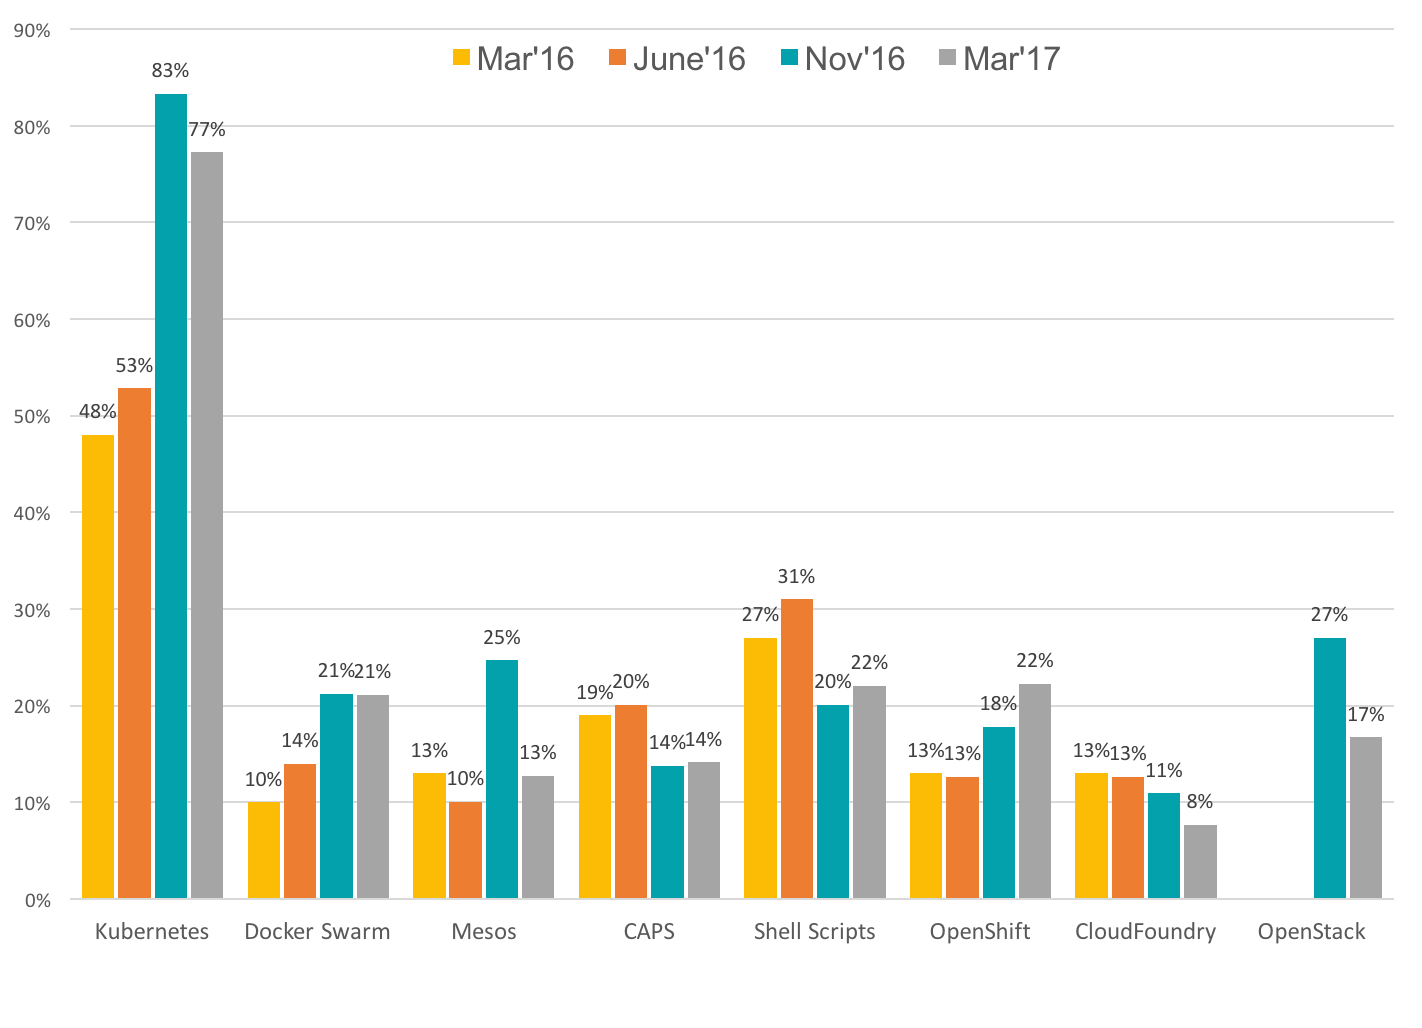
\includegraphics[width=14cm]{figures/cncf-container-orchestrators.png}
    \captionsetup{justification=centering,margin=2cm}
    \caption{Results of CNCF Survey from year 2017 showing Kubernetes as number one cloud management platform \cite{cncf-2017}}
    \label{fig:cncf-con}
\end{figure}



\subsection{Kubernetes architecture}
% this short summary before each subchapter helps me to stay focused on what i want to write about
\textit{This subchapter contains a high level description of the Kubernetes architecture. The focus is on the responsibilities of each Kubernetes component.}

\subsubsection{Kubernetes cluster}
A \textbf{Kubernetes cluster} may be defined as a collection of storage and networking resources which are used by Kubernetes to run various workloads \cite{book-mastering-k8s}. Another definition states that a Kubernetes cluster is a single unit of computers which are connected to work together and which are provisioned with Kubernetes components \cite{k8s-cluster}.

A cluster consists of two kinds of instances: masters and nodes. An instance can be a virtual machine or a physical computer \cite{article-k8s-as-avail,k8s-cluster}. This is depicted in figure ~\ref{fig:cluster-k8s}. Kubernetes nodes communicate with Kubernetes master.
\begin{figure}[H]
    \centering
    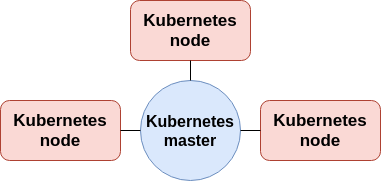
\includegraphics[width=10cm]{figures/cluster-k8s.png}
    \caption{Kubernetes cluster diagram depicting a master-slave architecture}
    \label{fig:cluster-k8s}
\end{figure}

\subsubsection{Masters and nodes}
\textbf{The role of the master is to manage the cluster}. This means that master: schedules applications, maintains their desired state, scales them, handles events, manages nodes. \textbf{Nodes serve as the worker machines}. They are responsible for running containers and handling container operations. Masters schedule containers to run on nodes \cite{book-mastering-k8s, k8s-cluster}. At least one node and one master is needed in a Kubernetes cluster. In order to provide fault-tolerance and high availability in production environments, multiple master and multiple node instances are run \cite{k8s-components}.

The instances in a Kubernetes cluster (masters and nodes) are hosts to several \textbf{Kubernetes components}. There are \textbf{master components}, used to control the cluster and there are also \textbf{node components}, run on each node. All the components are presented in figure \ref{fig:components-of-kubernetes}:
\begin{figure}[H]
    \centering
    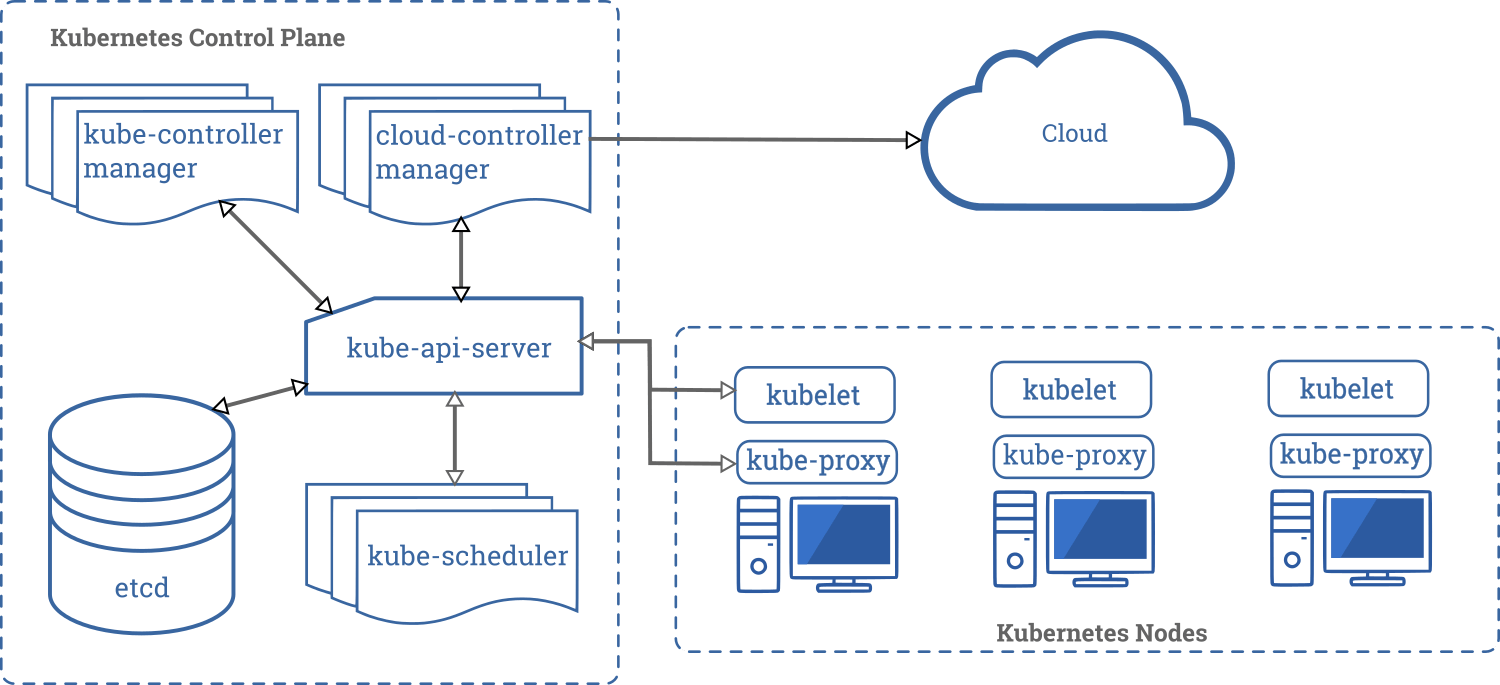
\includegraphics[width=14cm]{figures/components-of-kubernetes.png}
    \caption{Kubernetes components including master and node components \cite{k8s-components}}
    \label{fig:components-of-kubernetes}
\end{figure}


\subsubsection{Components}
The master components are also known as the control plane’s components. They are as follows \cite{book-mastering-k8s, k8s-components}:
\begin{itemize}
\item Etcd (a key-value store),
\item API server,
\item Scheduler,
\item Controller manager and Cloud Controller manager.
\end{itemize}

\paragraph{}
\textbf{Etcd} stores the entire cluster state. It is a highly-available key-value store. It is enough, for a test Kubernetes cluster, to deploy one instance of Etcd. However, for the purposes of high availability and redundancy, a 3-node or even 5-node Etcd cluster is typical. It is recommended to have a back up plan for the data stored in Etcd\cite{book-mastering-k8s,k8s-components}. The name \textit{etcd} follows a naming convention within the UNIX directory structure. In UNIX, all system configuration files are contained in a folder called "/etc". The last letter "d" stands for "distributed" \cite{etcd-name}.

\textbf{API server} exposes the Kubernetes REST API. It allows the nodes to communicate with the master and it also allows end users to interact with the cluster. Thanks to the fact that API server is stateless and that all its data is stored in etcd, API server can easily scale horizontally. The main implementation of a Kubernetes API server is kube-apiserver\cite{book-mastering-k8s,k8s-components,k8s-cluster}.


\textbf{Scheduler} is responsible for assiging containers to nodes. Scheduler selects a node for a container to run on. It considers a range of factors: resource requirements, various constraints, affinity and anti-affinity specifications, data locality, inter-workload interference, and deadlines. The implementation is known as kube-scheduler \cite{book-mastering-k8s, k8s-components}.

\textbf{Controller manager} runs controller processes such as: watching the shared state of the cluster and making changes needed to move the current state into the desired state. Controller manager is a collection of separate managers, but they are all compiled into a single binary and run in a single process in order to reduce complexity. The controllers consist of: Node Controller, Replication Controller, Endpoints Controller, Service Account and Token Controllers. The implementation of Controller manager is kube-controller-manager \cite{book-mastering-k8s, k8s-components}.

\textbf{Cloud Controller manager} interacts with a specified underlying cloud provider (e.g. Amazon Web Services or Google Cloud Platform). It is implemented by cloud-controller-manager and therefore, it allows the Kubernetes code and the cloud vendor’s code to evolve independently \cite{k8s-components}.

As aforementioned, there are also node components. They run on both: masters and nodes. They are as follows \cite{book-mastering-k8s, k8s-components}:
\begin{itemize}
\item Kubelet,
\item Proxy,
\item Container Runtime.
\end{itemize}

\textbf{Kubelet} oversees the communication with the master components (by monitoring API server for changes) and makes sure that containers, described by a Pod, are running and healthy (so it manages a Pod lifecycle). A Pod is a simple object from a Kubernetes API and it represents a set of containers. Containers which were not created by Kubenernetes are not managed by Kubelet \cite{book-mastering-k8s, k8s-components}.

\textbf{Proxy} is implemented by kube-proxy. It is a network proxy and it implements a part of the Kubernetes Service concept, which means that it is responsible for exposing an application as a network service and it provides load balancing \cite{book-mastering-k8s, k8s-components}.

\textbf{Container Runtime} is the software which is responsible for operating containers. Several container runtimes are supported: Docker, containerd, CRI-O, and any implementation of the Kubernetes CRI (Container Runtime Interface). It is a design policy of Kubernetes that is ought to be decoupled from a specific container runtime. Under some circumstates it should be possible to switch from one container runtime to another or to use multiple of them at once. Originally, Kubernetes was designed to manage only Docker containers \cite{book-mastering-k8s, k8s-components}.

\subsubsection{Other services}
\label{k8s-other-services}
Apart from master and node components, there are also \textbf{add-ons, extensions, and third party tools} which communicate with Kubernetes by the API server and which provide additional functionality. Examples of such services are: DNS, Vertical Pod Autoscaler, Cluster Autoscaler, Istio, Kubernetes Dashboard, kube-ops-view, node-problem-detector, etc \cite{book-cndwk}}.

\subsubsection{The Kubernetes networking model}
\label{k8s-net}
Kubernetes states a few \textbf{networking requirements} \cite{k8s-net}:
\begin{itemize}
\item pods on a node must be able to communicate with all pods on all nodes without Network Address Translation (NAT),
\item agents on a node (e.g. system daemons, kubelet) must be able to communicate with all pods on that node.
\end{itemize}

There are many available options that help with satisfying these requirements, e.g. AWS VPC CNI for Kubernetes, Azure CNI for Kubernetes, Flannel, OpenVSwitch, Project Calico, etc \cite{k8s-net}. CNI stands for Container Networking Interface and it is a specification and also a set of libraries for writing network plugins to configure network interfaces in Linux containers. A CNI container is bound to have its own IP address. For Kubernetes, \textbf{each pod has its own IP address}, so the pod is the CNI container \cite{book-mastering-k8s}. \textbf{Containers that belong to a one pod share the same IP address}, which means that these containers can reach all reach each other’s ports on localhost and also that none two containers should expose the same port. This model is known as "IP-per-pod" \cite{k8s-net}.

\subsection{Production deployment requirements}
\textit{This section explains what a production deployment is and what requirements it must met.}
~\\

\subsubsection{Multiple environments in software deployment}
First, it is helpful to distinguish between the terms: \textbf{'infrastructure stack' and 'environment'}. They both may be defined as a collection of infrastructure resources. The difference is that \textbf{an environment is conceptual, while a stack is concrete}. A stack is defined with code, particularly when Infrastructure as Code is applied, and managed using tools. However, an environment serves to fulfill a predetermined purpose. Multiple environments can run an instance of the same system\cite{book-iac}.

Typically, there are \textbf{two reasons for which multiple environments are in use}: to support a release delivery process and to run multiple production instances of the system. The first reason allows to have a particular build of an application (e.g. a git commit or a specified version of code) well tested. Such a build has to go through many different environments, e.g.: testing, staging and production. When a build does not pass all the stages in the former environments, it will not be promoted to the production environment\cite{book-iac}\cite{book-cicd}.

To briefly explain the second reason for multiple environments: they are used in order to ensure fault-tolerance (when one environment fails, the other can take over), scalability (the work can be spread among many clusters), segregation (it may be decided to handle a group of customers using one environment and the other group with the other environment, e.g. for latency purposes)\cite{book-iac}. Well-known examples of running multiple production deployments can be \textbf{Blue-green deployments or Canary deployments}\cite{bachelor-ha}.

\subsubsection{Production deployment requirements}
\label{Production deployment requirements}
Throughout this work a production deployment means such a deployment which targets the production environment. A list of \textbf{requirements for a production deployment}, gathered through the literature, is provided below:
\begin{itemize}
\item \textbf{Central Monitoring} - this is helpful when troubleshooting a cluster\cite{book-mastering-k8s}\cite{online-weave-checklists}\cite{online-weave-guide}\cite{book-cndwk}.
\item \textbf{Central Logging} - this is a fundamental requirement for any cluster with number of nodes or pods or containers greater than a couple\cite{book-mastering-k8s}\cite{online-weave-checklists}\cite{book-devops-k8s}.
\item \textbf{Audit} - to show who was responsible for what action\cite{online-weave-guide}.
\item \textbf{High Availability} - authors of \cite{book-mastering-k8s} go even further and state that the cluster should be tested for being reliable and highly available \textbf{before} it is deployed into production\cite{book-mastering-k8s}\cite{book-cndwk}.
\item \textbf{Live cluster upgrades} - it is not affordable for large Kubernetes clusters with many users to be offline for maintenance\\cite{book-mastering-k8s}.
\item \textbf{Backup, Distaster Recovery}\cite{book-mastering-k8s}\cite{online-weave-guide}\cite{book-cndwk}.
\item \textbf{Security, secrets management, image scanning} - security at many levels is needed (node, image, pod and container, etc.)\cite{book-mastering-k8s}\cite{online-weave-checklists}\cite{online-weave-guide}\cite{book-cndwk}.
\item \textbf{Passing tests, a healthy cluster} - 'if you don't test it, assume it doesn't work'\cite{book-mastering-k8s}\cite{book-cndwk}.
\item \textbf{Automation and Infrastructure as Code} - in production environment a versioned, auditable, and repeatable way to manage the infrastructure is needed\cite{book-mastering-k8s}\cite{online-weave-guide}.
\item \textbf{Autoscaling} - if application deployed on a Kubernetes demand more resources, then a new Kubernetes node should be automatically created and added to the cluster. However, autoscaling, even though nice to have, is not that important\cite{book-cndwk}.
\end{itemize}

\subsubsection{Monitoring as production environment requirement}
\textbf{Monitoring} helps to ensure that a cluster is operational, correctly configured and that there are enough resources deployed. Monitoring is also indispensable for debugging and troubleshooting\cite{book-mastering-k8s}. The third reason for using a monitoring system is that historical data is needed for planning purposes. The monitoring strategy should cover four areas\cite{book-cicd}:
\begin{itemize}
\item configuring the infrastructure in such a way that it is possible to collect the data,
\item storing the data,
\item providing dashboards, so that data is presented in a clear way,
\item setting up notifications or alarms to let people know about certain events.
\end{itemize}
\paragraph{}
Monitoring provides various \textbf{metrics}, e.g.: CPU usage, memory utilization, I/O per disk, disk space, number of network connections, response time, etc. Thus, it is helpful on many different levels: on hardware, operating system,  middleware and application level. There is a wide range of \textbf{available open source and commercial tools} to take care of monitoring: Nagios, OpenNMS, Flapjack, Zenoss, Tivoli from IBM, Operations Manager from HP, Splunk, etc.\cite{book-cicd}. Solutions recommended for a Kubernetes cluster are: Heapster combined with InfluxDB as backend and Grafana as frontend and also cAdvisor\cite{book-mastering-k8s}. A nice feature of Grafana are its dashboards. Example Grafana dashboard is presented in the next image:
\begin{figure}[H]
  \centering
  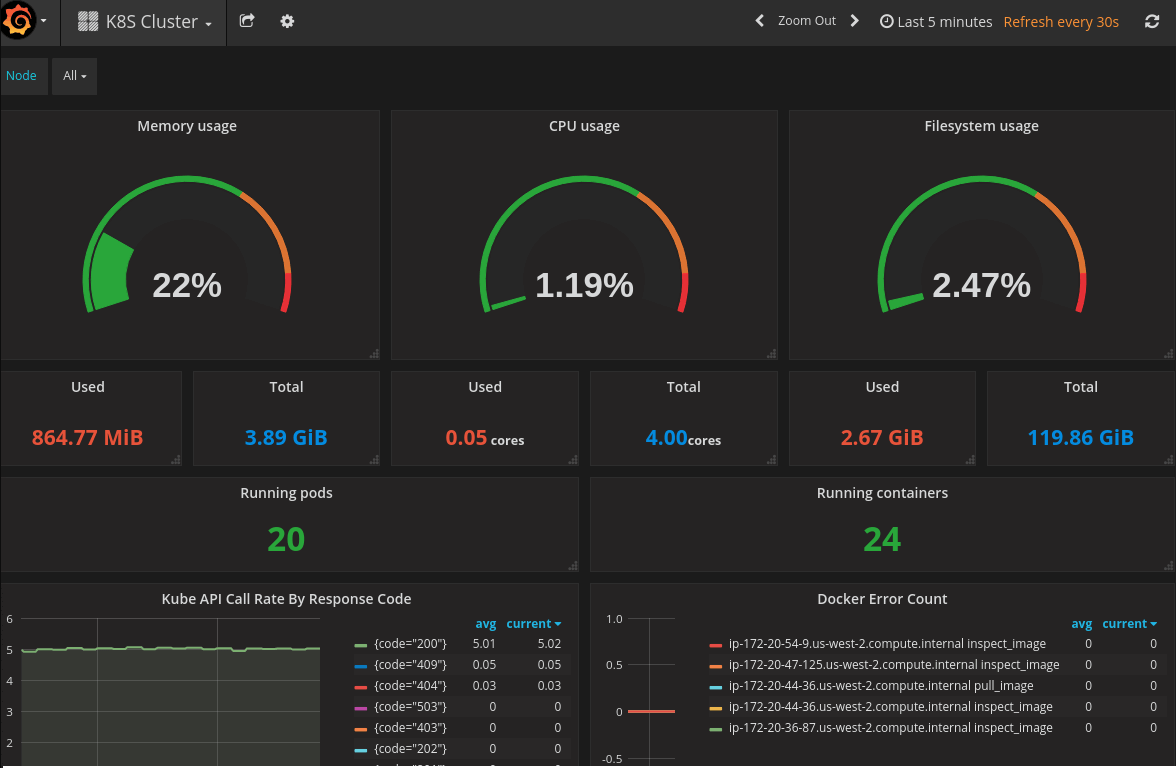
\includegraphics[width=11cm]{figures/grafana.png}
  \label{fig:grafana}
  \caption{Example Grafana dashboard for a Kubernetes cluster, showing among others: Memory, CPU and File system usage\cite{monitor-kubernetes-cluster-prometheus-grafana}}
\end{figure}
Grafana also works well with Prometheus, which is a monitoring system and a time series database. Prometheus is also a CNCF graduated project\cite{online-prometheus-gh}\cite{online-prometheus-www}. If a system (like Kubernetes) is deployed on AWS, another solution for monitoring and logging may be: Amazon CloudWatch\cite{online-cw}.

Another solution for monitoring is Kubernetes dashboard, which is a built-in solution and doesn't require any customization. Heapster, InfluxDB and Grafana are great for heavy-duty purposes, whereas Kubernetes dashboard is probably able to satisfy the majority of monitoring needs of a Kubernetes cluster\cite{book-mastering-k8s}\cite{book-devops-k8s}. Example dashboard provided by Kubernetes dashboard is depicted on the next image:
\begin{figure}[H]
  \centering
  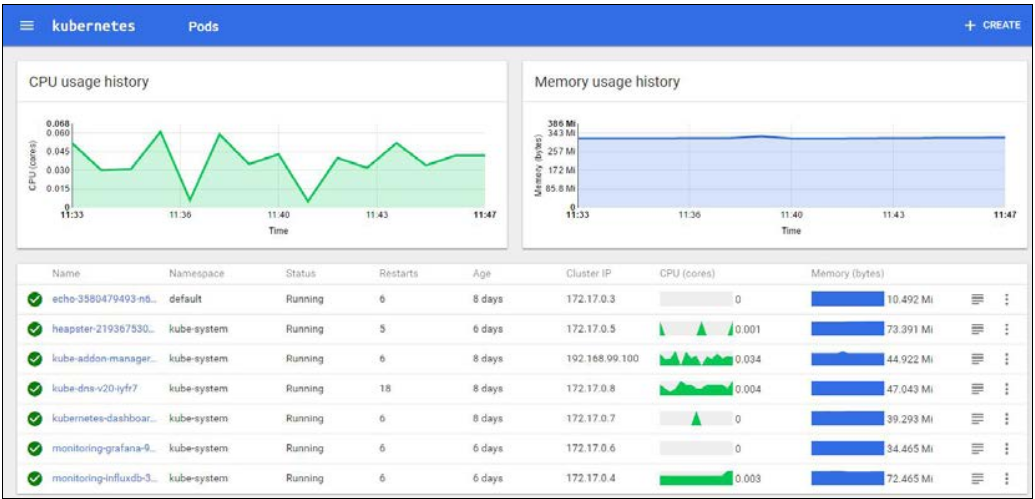
\includegraphics[width=10cm]{figures/k8s-dashboard.png}
  \caption{Kubernetes dashboard depicting CPU and Memory usage by Kubernetes pods\cite{book-mastering-k8s}}
\end{figure}

\subsubsection{Logging as production environment requirement}
Kubernetes dashboard has also a feature which makes it able to show \textbf{log messages} of a single container deployed on Kubernetes\cite{book-mastering-k8s}. \textbf{Centralized logging} is essential for a production cluster, because usually there are a lot of pods (and containers) deployed, each generating many log messages. It is impossible to require a Kubernetes administrator to login into each container for the purpose of getting the logs.

The second reason for the importance of centralized logging is that \textbf{containers are ephemeral} - the log messages kept inside the containers would be lost after a container is redeployed. \textbf{Popular solutions} are: Fluentd, Elasticsearch, Kibana\cite{book-mastering-k8s}, Logstash\cite{book-devops-k8s} and Graylog\cite{online-prod-year-k8s}\cite{online-graylog}. It is also important to consider that log messages in Kubernetes cluster are generated from many sources: from end-user applications, nodes, Kubernetes system containers and there are also \textbf{audit logs} in the form of e.g. api server events\cite{online-graylog-art}. For the purposes of auditing, when deploying on AWS, one can use AWS CloudTrail\cite{online-ct}.

\subsubsection{High Availability as production environment requirement}
While administering a Kubernetes cluster, there is a high probability that something will go wrong. Components, network can fail, configuration can be incorrect, people make mistakes and software has bugs. Failure classification has been described in \cite{article-failures}. This has to be accepted and a system should be designed in such a way that it is \textbf{reliable and highly available (HA)} despite of many problems. Here is a list of ideas how to ensure high availability\cite{book-mastering-k8s}:
\begin{itemize}
\item \textbf{Redundancy} - means having a spare copy of something. Kubernetes uses Replica Sets or Replication Controllers to provide redundancy for applications deployed on Kubernetes. Five redundancy models were summarized in \cite{article-redundancy-models}. Some of them require an active replica (running) and other passive (or standby).
\item \textbf{Hot Swapping} - can be explained as replacing some failed component on the fly, with minimal or ideally zero down-time. Actually, hot swapping is quite easy to implement for stateless applications. For stateful applications, one has to keep a replica of a component (see redundancy).
\item \textbf{Leader election} - it is a pattern used in distributed systems. Whenever there are many servers fulfilling the same purpose to share the load. One of the servers must be elected a leader then and certain operations must go through it. When the leader server experiences a failure, other server can be selected as new leader. This is a combination of redundancy and hot swapping.
\item \textbf{Smart load balancing} - used to share and distribute the load.
\item \textbf{Idempotency} - means that one request (or some operation) is handled exactly once.
\item \textbf{Self-healing} - means that whenever a failure of one component happens, it is automatically detected and steps are taken (also automatically) to get rid of the failure.
\item \textbf{Deploying in a cloud} - a goal is to be able to physically remove or replace a piece of hardware, either because of some issues or because of preventative maintenance or horizontal growth. Often this is too expensive or even impossible to achieve\cite{article-failures}. Traditional deployments on-premises forced administrators to do a capacity planning (to predict the amount of computing resources). Thanks to the on-demand and elastic nature of the clouds, the infrastructure can be closely aligned to the actual demand. It is also easy to scale applications deployed on a cloud, because of the fundamental property of the cloud: elasticity\cite{article-aws-architecting}.
\end{itemize}

Generally speaking, \textbf{"highly available systems are fault tolerant systems with no single point of failure"}\cite{article-redundancy-models}. In order to introduce HA for the Kubernetes cluster the following ideas could be incorporated\cite{book-mastering-k8s}:
\begin{itemize}
\item Deploy Etcd as a cluster, not just one instance of Etcd.
\item Ensure redundancy for api server.
\item Deploy multiple master instances and ensure a load balancer in front of them.
\item Ensure that node instances are reliable: the Docker daemon and the Kubelet daemon should restart automatically in case of failure.
\item Apply RAID to ensure redundancy of data storage or apply Key-Value Multi-Device (KVMD), a hybrid data reliability manager\cite{data-rel-kv} or let cloud provide storage availability.
\end{itemize}

Furthermore, it may be needed to test high availability. This can be done by inducing a predictable failure and verifying if the system behaves as expected\cite{book-mastering-k8s}. Such a kind of testing, where one or more cluster nodes or pods is killed is called Chaos Monkey, after the tool developed by Netflix. There are also ready to use tools basing on the idea of Chaos Monkey: chaoskube, kube-monkey, PowerfulSeal\cite{book-cndwk}.
\begin{figure}[H]
    \centering
    
\includegraphics[width=3cm]{figures/chaos-monkey-logo.png}
    \label{fig:chaos-monkey-logo}
    \caption{Logo of the Netflix program: Chaos Monkey\cite{chaosmonkey}}
\end{figure}

\subsubsection{Automation as production environment requirements}
\label{Automation as production environment requirements}
When it comes to \textbf{automation}, many guidelines can be found in \cite{book-cicd}. Below are some of them listed:
\begin{itemize}
\item \textbf{Every Change Should Trigger the Feedback Process} - means that every change in code should trigger some pipeline and should be tested (including unit tests, functional acceptance tests, nonfunctional tests). The tests should happen in an environment which is as similar as possible to production. Some tests may run in production environment too\cite{book-cicd}\cite{book-iac}.
\item \textbf{The Feedback Must Be Received as Soon as Possible} - this also involves another rule: fail fast. This guideline suggests that faster tests (or less resource-intensive tests) should run first. If theses tests fail, the code does not get promoted to the next pipeline stages, which ensures optimal use of resources\cite{book-cicd}.
\item \textbf{Automate Almost Everything} - generally, the build process should be automated to such extent where specific human intervention or decision is needed. But there is no need to automate everything at once\cite{book-cicd}\cite{book-iac}.
\item \textbf{Keep Everything in Version Control} - this means that not only application source code but also tests, documentation, database configuration, deployment scripts, etc. should be kept in version control and that it should be possible to identify the relevant version. Furthermore, any person with access to the source code should be able to invoke a single command in order to build and deploy the application to any accessible environment. Apart from that, it should be also clear which version in version control was deployed into each environment\cite{book-cicd}.
\item \textbf{If It Hurts, Do It More Frequently, and Bring the Pain Forward} - if some part of the application lifecycle is painful, it should be done more often, certainly not left to do at the end of the project\cite{book-cicd}.
\item \textbf{Idempotency} - the tools used for automation should be idempotent, which means that no matter how many times the tool is invoked, the result should stay the same\cite{book-iac}.
\end{itemize}

\paragraph{}
Together with automation, there are two inextricably entwined terms: Infrastructure as Code and DevOps. As these two terms has been already explained in this work, now let us focus on the essential tools needed to introduce the automated application lifecycle. First, a framework for \textbf{Configuration Management} is needed. Examples involve: Puppet, CFEngine\cite{book-cicd}\cite{book-iac}, Chef\cite{online-chef}, Ansible\cite{online-ansible}, SaltStack\cite{online-salt}, etc. These tools help to declaratively define what packages should be installed and how should they be configured in a virtual machine or a container or a physical server\cite{book-cicd}. They can help prevent \textbf{configuration drift} in a large number of computers\cite{book-devops-k8s}. A configuration drift is a difference across systems that were once identical. It can be imposed by a manual amendment and also by automation tools which propagated a change only to some of the instances\cite{book-iac}. There are also stack-oriented tools, which follow the same declarative model: Terraform\cite{terraform} and CloudFormation\cite{book-iac}. Another type of needed tools is a building server, examples are: Jenkins, GoCD, Travis - they were already mentioned earlier.

\subsubsection{Security as production environment requirement}
\textbf{Security} is another essential aspect of production deployment and, as mentioned above, it touches many levels. A node breach is a very serious problem and it can happen by someone logging to the instance or having physical access to it. The latter is easily mitigated by not deploying on bare-metal machines but on a cloud instead\cite{book-mastering-k8s}. The former demands some hardening done. There are several ideas that can be implemented for a Kubernetes cluster specifically listed below:
\begin{itemize}
\item ensuring that data is encrypted in transit by using secure api server protocol (HTTPS instead of HTTP)\cite{book-mastering-k8s}.
\item ensuring proper user and permissions management by configuring authentication, authorization, security accounts and admission control in api server \cite{book-mastering-k8s}. When setting up authorization, it is wise to apply \textbf{the principle of least privilege}. This principle recommends that only the needed resources or permissions should be granted\cite{book-cndwk}.
\item utilizing Role-Based Access Control (RBAC) to manage access to a cluster\cite{book-cndwk}.
\item ensuring security keys management and exchange\cite{book-mastering-k8s} by implementing for example automated key rotation.
\item ensuring that used Docker images are neither malicious (deliberately causing some harm) nor vulnerable (allowing some attacker to take control) by keeping them up-to-date and maintaining them instead of using the publicly available ones or by using a private Docker registry\cite{book-mastering-k8s}.
\item using minimal Docker images because the fewer programs there are installed in an image, the fewer potential vulnerabilities there are\cite{book-cndwk}.
\item maintaining a log or audit system\cite{book-mastering-k8s}.
\item utilizing network policies which act in a whitelist fashion and can open certain protocols and ports\cite{book-mastering-k8s}.
\item using secrets. Kubernetes has a resource called: secret, but the problem is, that Kubernetes stores secrets as plaintext in Etcd. This, in turn, means that steps should be taken in order to limit direct access to Etcd\cite{book-mastering-k8s}.
\item prefering managed services, because they will have many security measures already implemented\cite{book-cndwk}.
\item avoid running processes as root user in Docker containers\cite{book-cndwk}.
\item using available programs for security scanning\cite{book-cndwk}.
\end{itemize}

The following illustration presents security features provided by Kubernetes API server:
\begin{figure}[H]
    \centering
    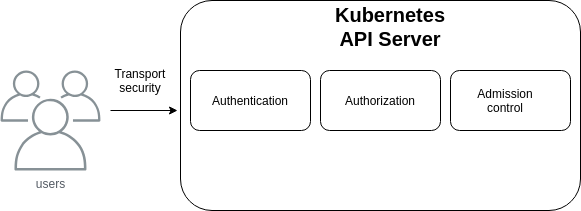
\includegraphics[width=13cm]{figures/api-server-security.png}
    \label{fig:security-api-server}
    \caption{Security features which a request sent to Kubernetes API Server goes through. Based on the official documentation website\cite{k8s-sec}}
\end{figure}

There are many more security measures that Kubernetes administrators and end-users could apply. A curious reader is referred to\cite{book-cndwk} and \cite{book-mastering-k8s}.

\subsubsection{Disaster recovery as production environment requirement}
\textbf{Disaster recovery} can be understood as the process which an organization has to undergo after a service  disruption happened in order to resume normal services. It is vital to know what actions are necessary to overcome the disaster. This set of predefined procedures is known as \textbf{Disaster Recovery Plan}. Furthermore, disaster recovery is not the same as fault tolerance. The latter ensures that a system will withstand and resist the failure\cite{article-dr}.

Disaster recovery is an essential requirement of any business where continuity matters. In order to plan disaster recovery well the following key parameters should be considered: the initial cost, the cost of data transfers and the cost of data storage. Significant costs may be a reason why, in the past, around 40-50\% of small businesses had no DRP and did not intend to change this. However, cloud computing provides affordable solutions, because of the employed model "pay-for-what is used". Another \textbf{advantage of the cloud is that it is fairly easy to use resources deployed in multiple geographical areas}. This is desired, because one the major concepts in a DRP is the geographical separation of the system servers and its backup\cite{article-dr-cloud}.

Key metrics that can be taken into consideration while planning disaster recovery are\cite{article-dr}\cite{article-dr-cloud}:
\begin{itemize}
\item Recovery Point Objective (RPO)
\item Recovery Time Objective (RTO)
\end{itemize}
\textbf{RPO} can be defined as the time between two successive backups. Thus, the time between the last backup and the the disaster, which is de facto the time of data loss, is maximally equal to RPO. \textbf{RTO} can be understood as the time needed to recover from the disaster, when the server experiences downtime\cite{article-dr-cloud}. RPO and RTO are illustrated on the following image:
\begin{figure}[H]
    \centering
    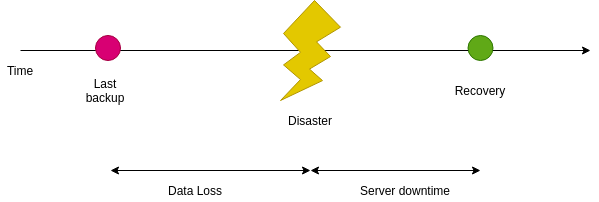
\includegraphics[width=13cm]{figures/rpo-rto.png}
    \label{fig:rpo-rto}
    \caption{RPO and RTO illustrated in relation to time}
\end{figure}

Cloud services mitigate some risks that persistent data storage has. For example: cloud services provide high-available data storage by replicating it across different geographical locations. However, replication is not the same as backup and it does not protect against accidentally deleting a volume or against a misconfigured application overwriting the data. Thus, backup is still needed. In order to backup Kubernetes, the Etcd database has to be backuped. Apart from that, each application deployed on top of Kubernetes should be backuped on its own\cite{book-cndwk}. There are already available services that help with Kubernetes backup: Velero\cite{book-cndwk}.

\subsubsection{Testing as production environment requirement}
Before the production Kubernetes cluster is ready for end-users, it must be verified that \textbf{it works and is healthy}. Every component and every node should be tested proving that it is working as expected. Sometimes, applications expose a custom \textbf{health endpoint}\cite{book-devops-k8s}. E.g. kube-scheduler does that. Thanks to that, it is possible to verify regularly that a service is performing correctly by sending a request to the health endpoint. Usually, a HTTP response code of 200 indicates correct status of the service\cite{online-ms-health}. Kubernetes can monitor the health endpoints with \textbf{liveness probes}. Based on a specified health endpoint response, Kubernetes can restart the faulty container\cite{online-k8s-probes}.

The tests should be incorporated into a CICD pipeline. "Having a comprehensive test suite is essential to continuous integration" and test-driven development is a vital practice in this context\cite{book-cicd}. There is even a possibility to implement \textbf{test-driven} changes to deployment environments. The recipe for achieving that is described in "Continuous Delivery: Reliable Software Releases through Build, Test, and Deployment Automation"\cite{book-cicd}.

\newpage

% 3
\mysec{Available Kubernetes cluster deployment methods}
\newpage

% 4
\mysec{Preparations for production deployment of Kubernetes cluster}
% 4
\textit{This is a practical section. It includes planning and designing the production deployment, considering: capacity planning, choosing which requirements to satisfy and taking any other deployment and infrastructure related decisions.}
~\\

\subsection{Chosen requirements of production deployment}
\textbf{There are numerous requirements for a production deployment of a Kubernetes cluster}. Some of them were gathered throughout available literature and presented in the section: \ref{Production deployment requirements}. It is common knowledge that companies, which deploy Kubernetes and similar systems, obey some set of best practices, dedicated to these companies only. Thus, the requirements presented in this work do not exhaust the topic.

MAYBE TODO:
Furthermore, the author if this work decided to satisfy only a few of the production deployment requirements. The reason - because i don't want to.

\begin{itemize}
\item Passing tests, a healthy cluster
\item Automation and Infrastructure as Code
\item Central Monitoring
\item Central Logging
\item Backup
\item HA - maybe
\item Autoscaling - maybe
\item Security - maybe
\item Live Cluster Upgrades - rather not
\item Audit - rather not
\end{itemize}

\subsubsection{Designing automated tests}

\subsection{Capacity planning}
Virtualization and chicken-counting (0, 1, many) are your friends here. Virtu-
alization makes it easy to create an environment that represents the important
aspects of your production environment, while being able to run on a single
physical machine. Chicken-counting means that if your production site has
250 web servers, 2 should be enough to represent the significant process
boundaries. book-cicd, p. 254

\subsection{Other decisions and configuration}

\subsection{Expected cost}



troubleshooting k8s -mastering k8s p. 58

\newpage

% 5
\mysec{Production deployment of Kubernetes cluster, using various methods}
\newpage

% 6
\mysec{Comparison of the used methods}
\newpage

% 7
\mysec{Summary}
\newpage

\printbibliography[type=book,title={Books only}]
\printbibliography[type=article,title={Articles only}]
\printbibliography[nottype=book,nottype=article,title={Other sources}]

\end{document}
